\vspace*{5cm}
\begin{center}{\LARGE\bf Appendix A : Timeline Chart}\end{center}
\newpage
\setcounter{figure}{0}\renewcommand{\thefigure}{A.\arabic{figure}}
Both charts follow the department's Project Interaction Sheet (Second Half of 2026 and First Half of 2027). Figure~\ref{fig:timeline} lists every entry of the sheet with its date and status; weeks 0--7 are signed by the guide. Figure~\ref{fig:gantt} shows the same plan as a Gantt chart. As the sheet requires, implementation is split into four sections: (1) the causal engine core and the chat application base, (2) the evidence search (RAG), secondary outcomes and the website, (3) the causal engine and RAG inside the chat application, and (4) better retrieval, a real-data adapter and the evaluation tools. Diamonds mark the sheet's checks (25\% by 23 September, 40\% by 7 October, 60\% by 14 October, 80\% by 21 October); the team's own target for all four sections is 6 October. Dashed lines mark Synopsis Presentations I (12 August) and II (30 September 2026).
\begin{figure}[H]\centering
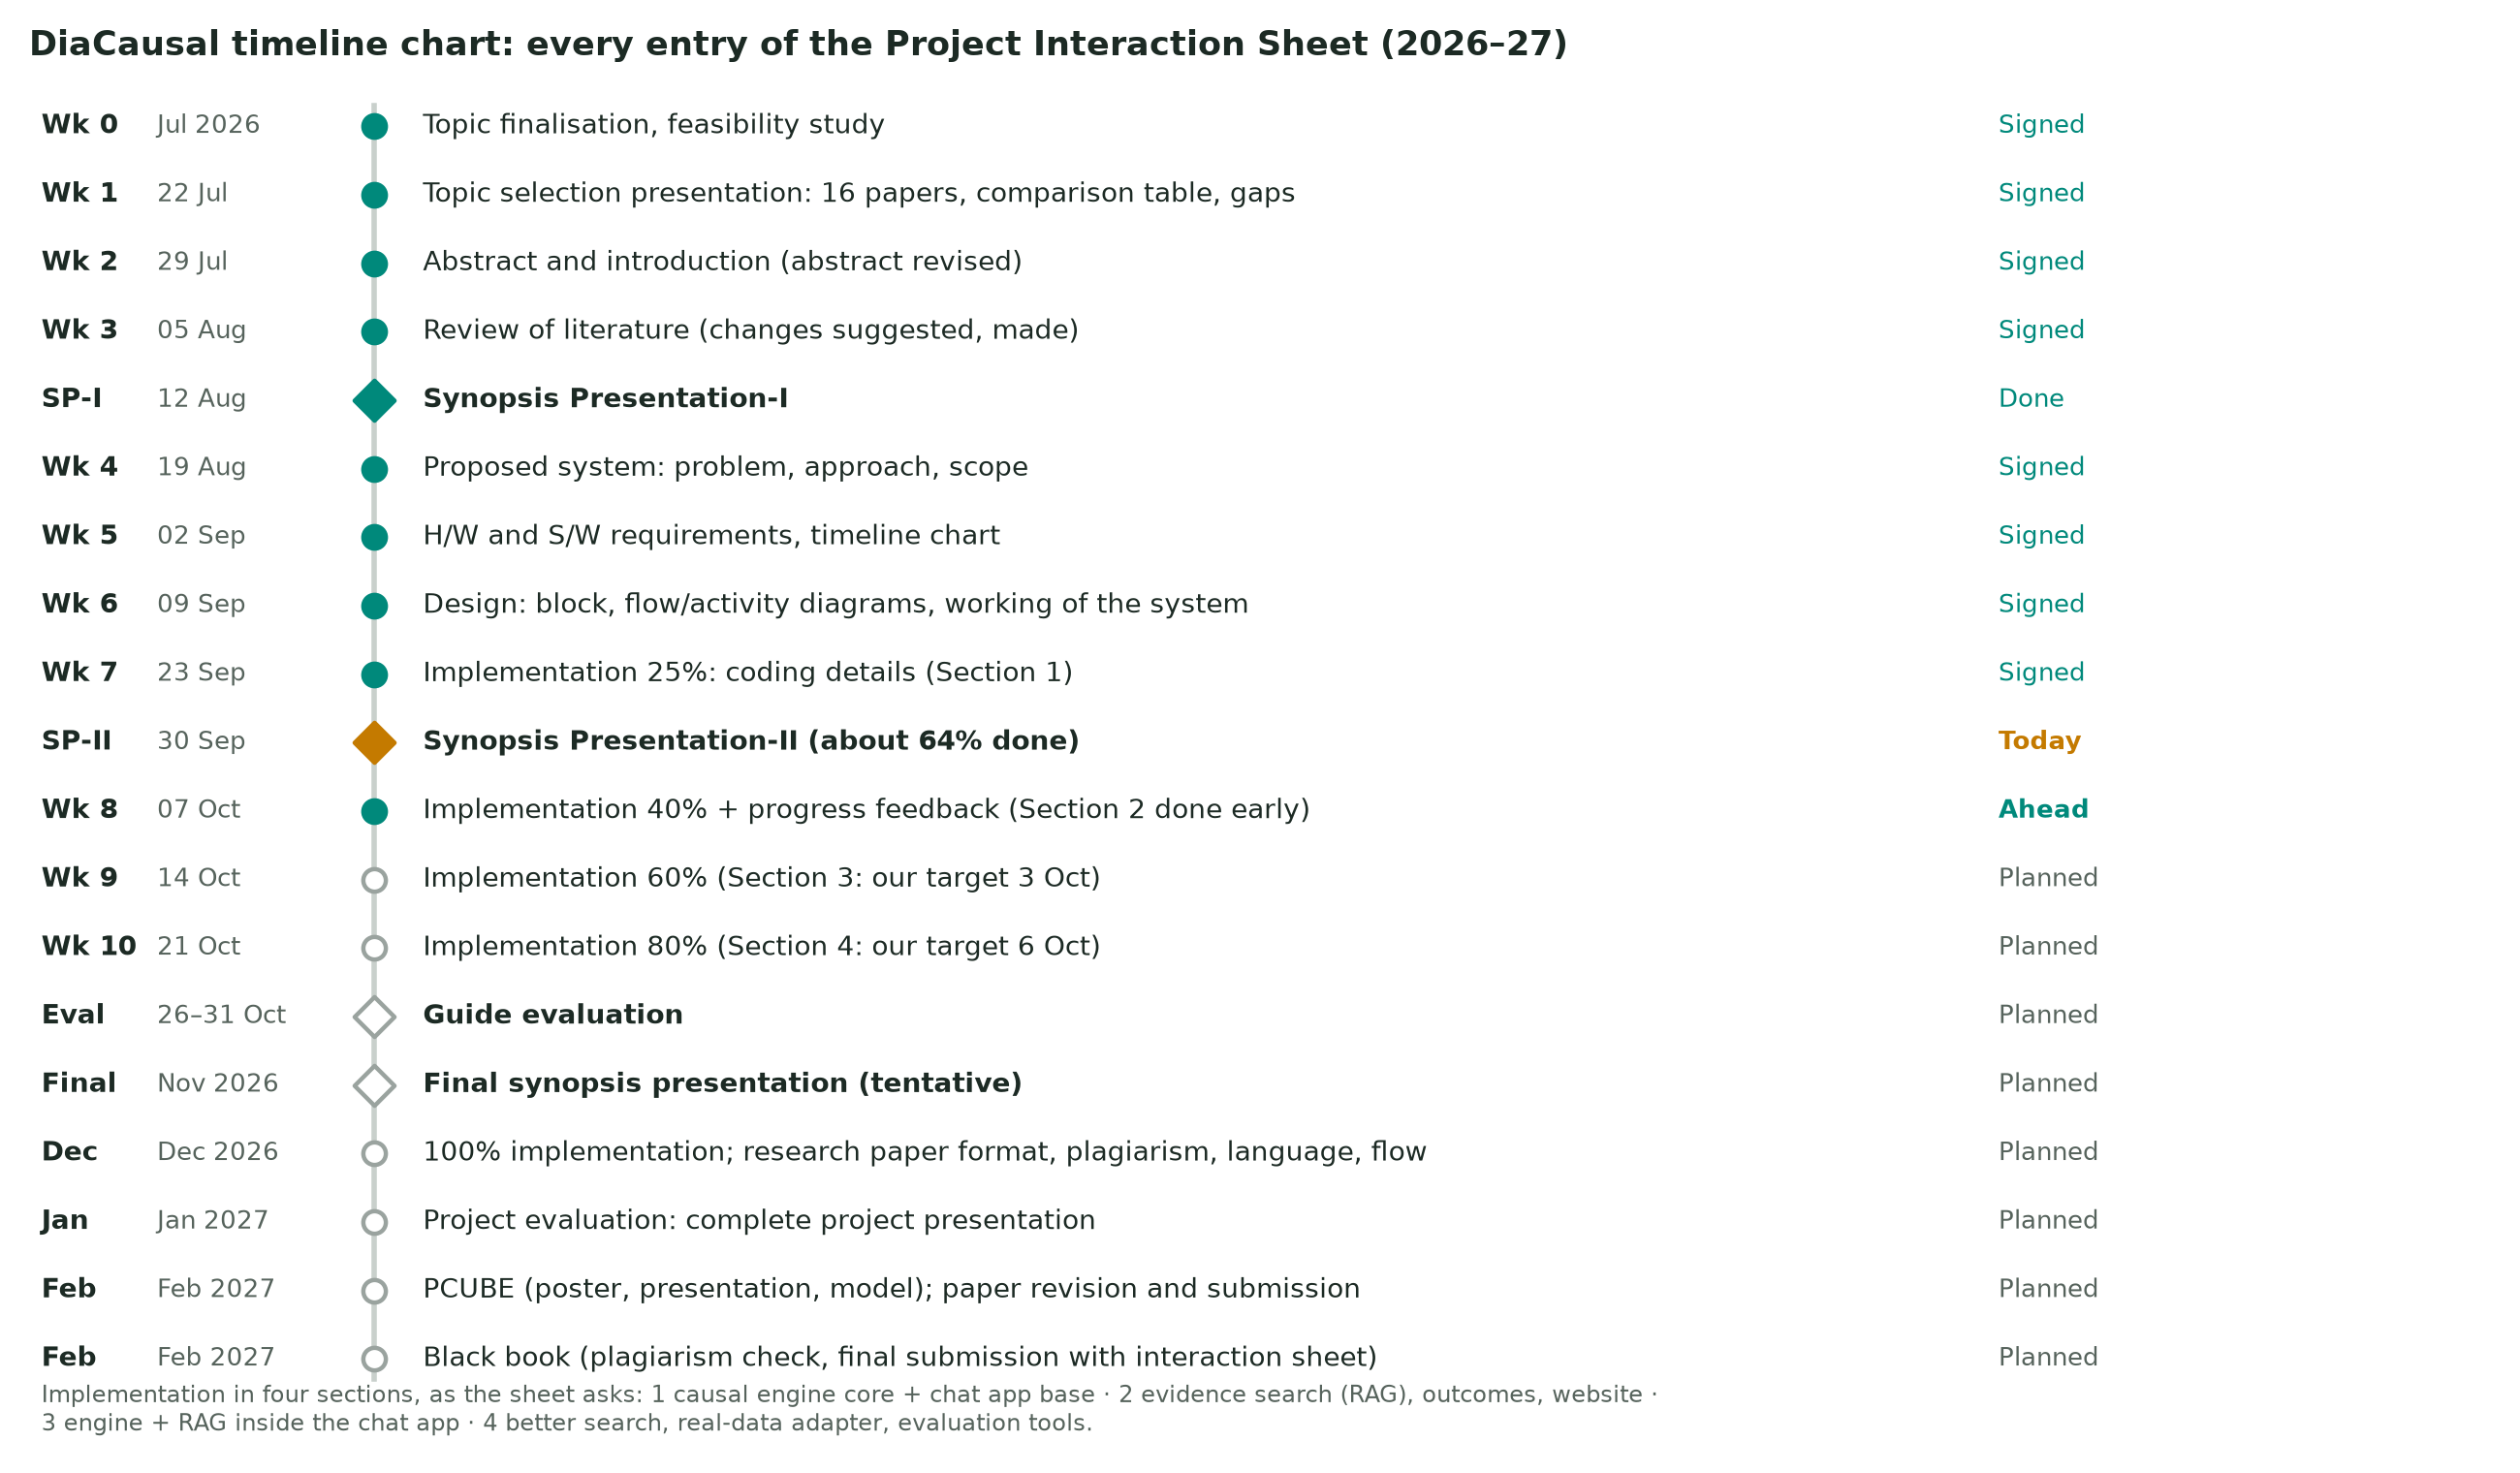
\includegraphics[width=\textwidth]{figures/timeline.png}
\caption{Timeline chart: every entry of the Project Interaction Sheet (2026--27)}\label{fig:timeline}\end{figure}
\begin{figure}[H]\centering
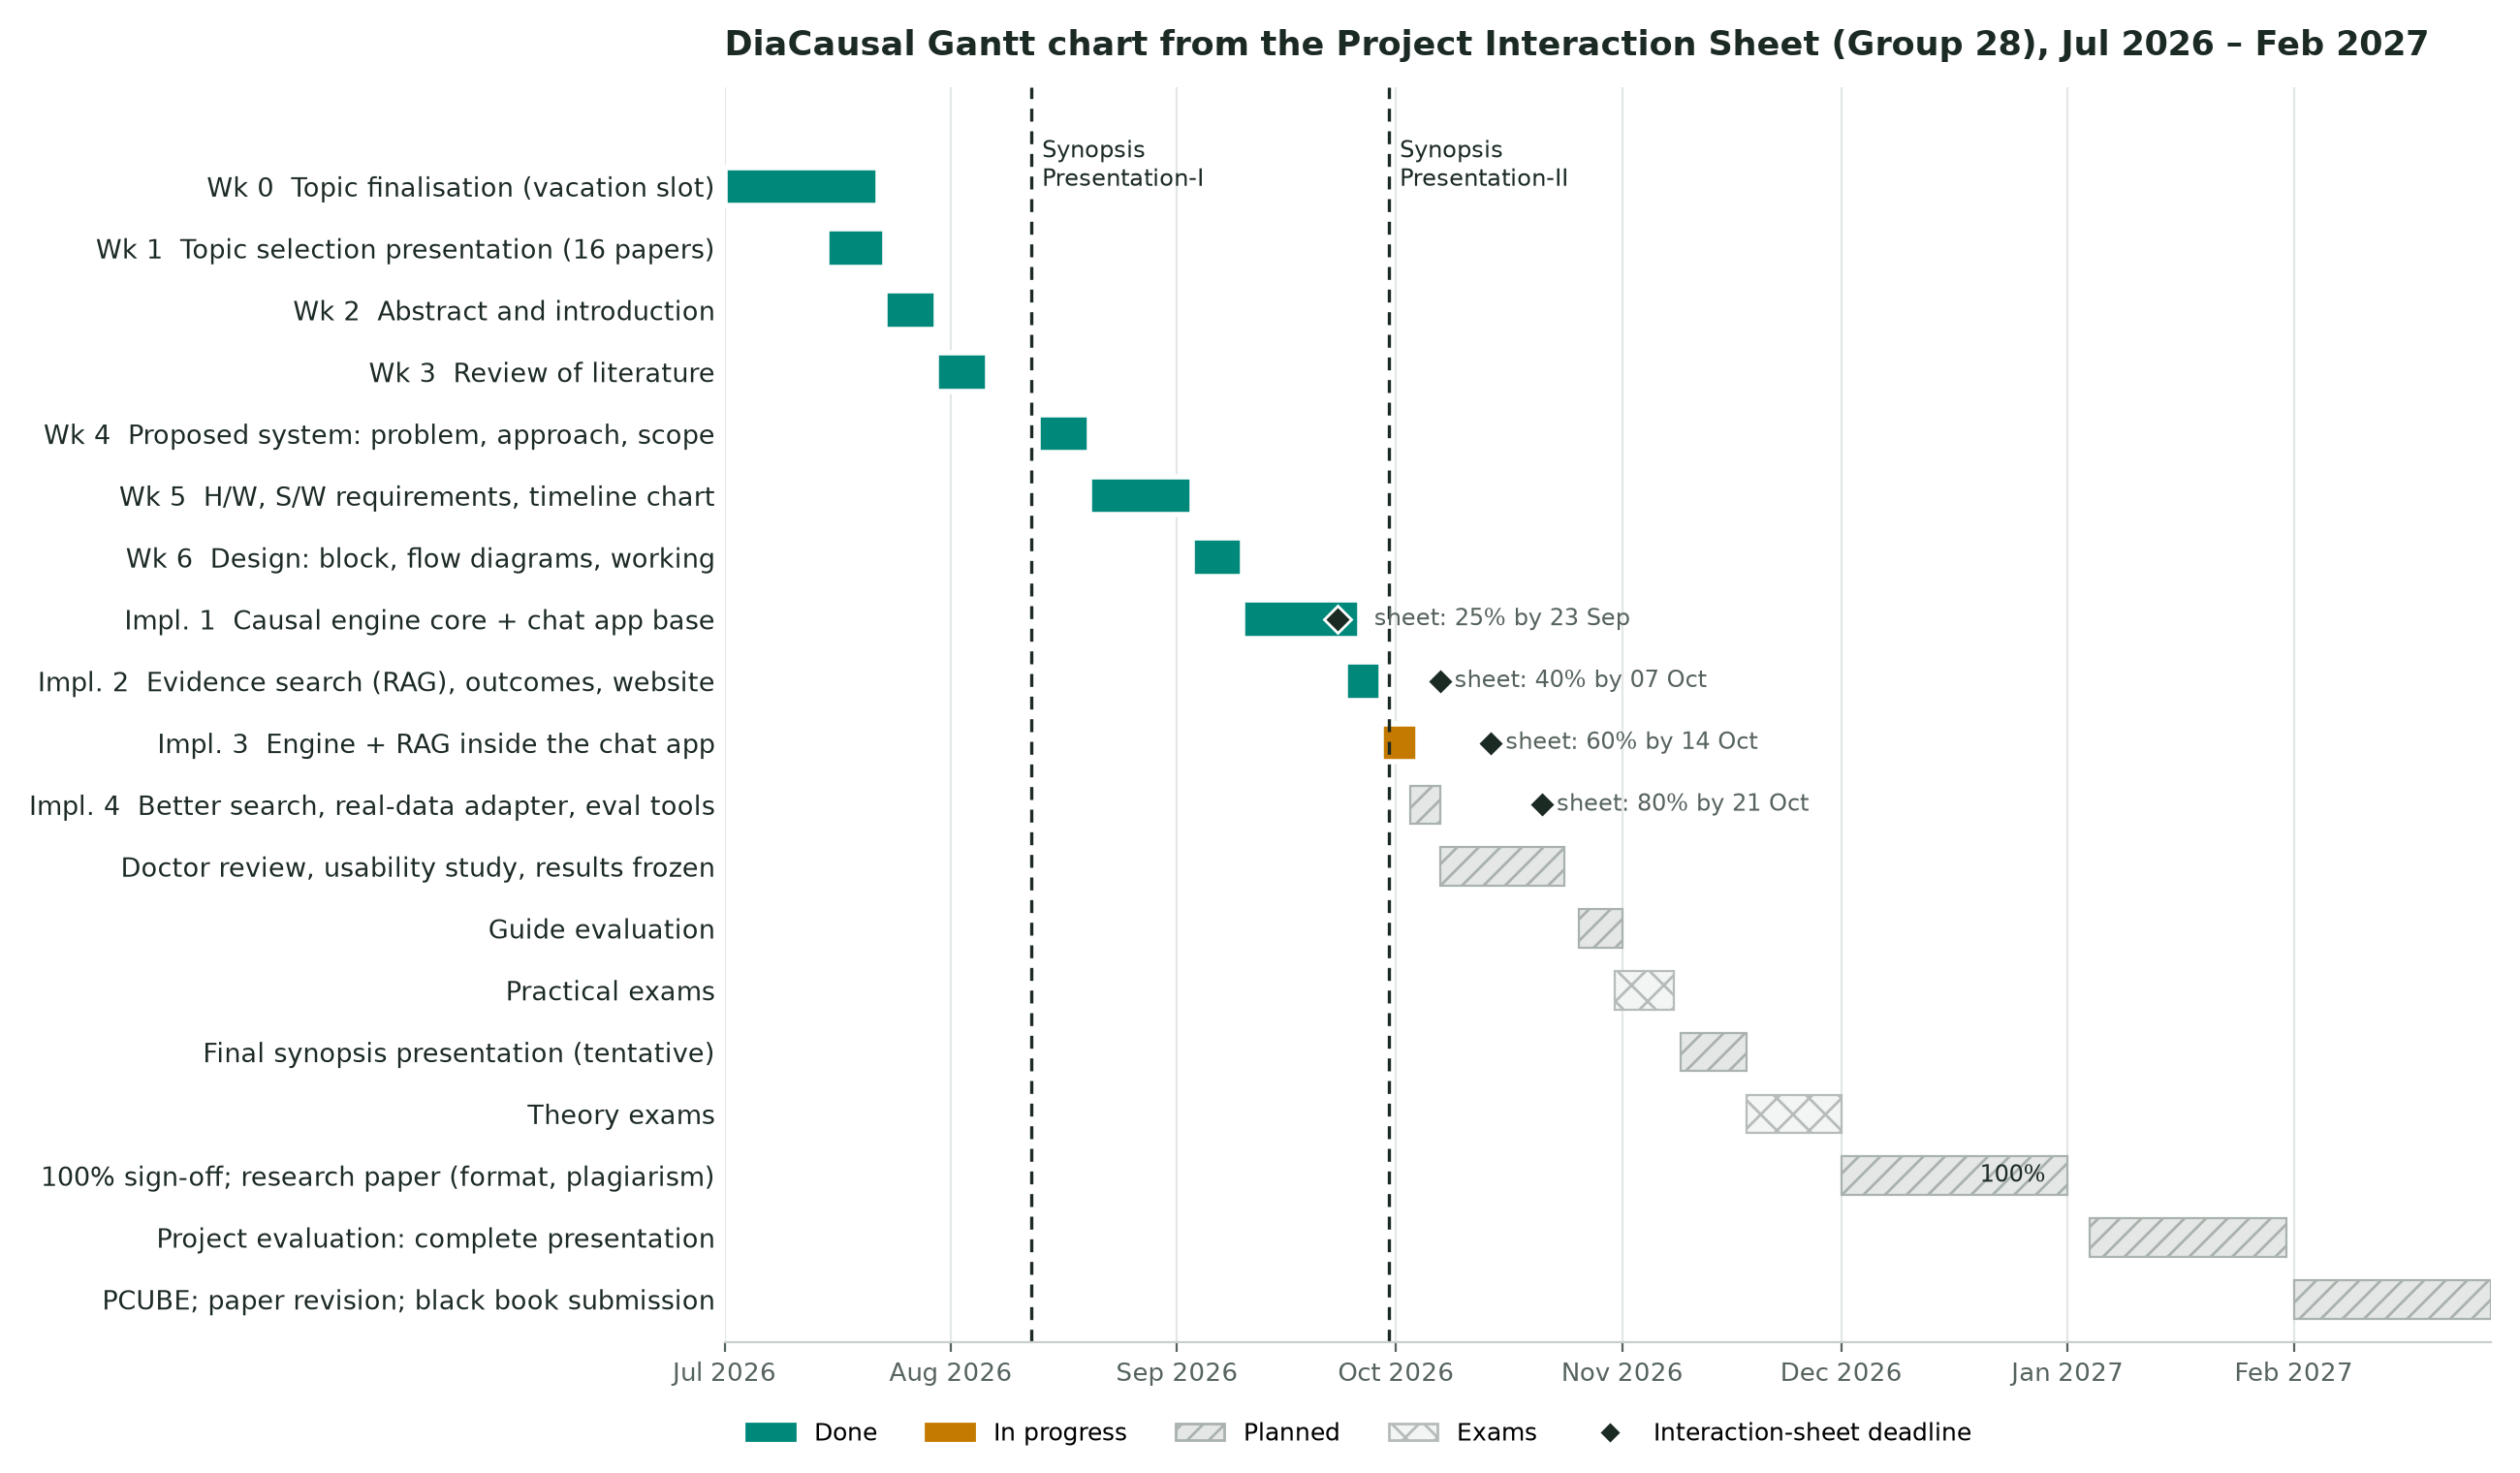
\includegraphics[width=\textwidth]{figures/gantt.png}
\caption{Gantt chart from the Project Interaction Sheet (July 2026--February 2027)}\label{fig:gantt}\end{figure}
